\subsection{NIC-Driven Thread Scheduling}
\label{ssec:thread-scheduler}
In some specialized applications, thread scheduling might not be needed: Big HPC applications, for example, might pin every nanotask to a dedicated core for the duration of a run.
But this would not work for a cloud provider who needs more economical sharing of \name{}s by multiple nanoservice applications.
Nanotask threads will therefore need to be switched in and out frequently, and context switches must be extremely fast, else we will lose all the low latency benefits of nanoservices.

If \name{} relied on software scheduling it would be too slow. 
The fastest best-of-breed software schedulers use 5$\mu$s timer interrupts~\cite{shinjuku, shenango} which are much too slow for our $<1\mu$s nanotasks.
And so, instead, the \name{} decides which thread to run next in hardware on the NIC (\Cref{fig:nanoPU}d), then tells the CPU core. 
The NIC keeps track of the highest-priority nanotask with messages to process and interrupts the CPU to initiate a context switch under two conditions:

\begin{enumerate}
    \item A message arrives for a higher priority context than the one currently running on the core.
    \item The current context tells the NIC it is idle, and the NIC has messages for another context to process. 
    This condition prevents an idle high-priority context from starving a low-priority context with messages waiting to be processed.
\end{enumerate}

\Cref{fig:nic-scheduler} shows what happens when a message arrives for a higher-priority context than the one currently running on the core. 
In step \ballnumber{a}, the arriving message is enqueued into the RX queue for the high-priority context.
In step \ballnumber{b}, the thread scheduler tells the CPU that a high-priority message is waiting by updating the \verb|ltargetcontext| CSR and firing an interrupt.
The interrupt causes a trap into the nanokernel, which then reads the \verb|ltargetcontext| CSR and performs a switch to the high-priority context in step \ballnumber{c}, updating the \verb|lcurcontext| CSR.
At this point, the high-priority context is running on the core and is able to process the message in its RX queue.
When the high-priority context finishes processing the message, it tells the NIC that it is now idle by writing to a dedicated CSR called \verb|lidle|.
The NIC then initiates a context switch back to the low-priority context because it still has messages to process.

\shahbaz{will update Figure~\ref{fig:nic-scheduler} to contain the relevant CSRs}

\begin{figure}
  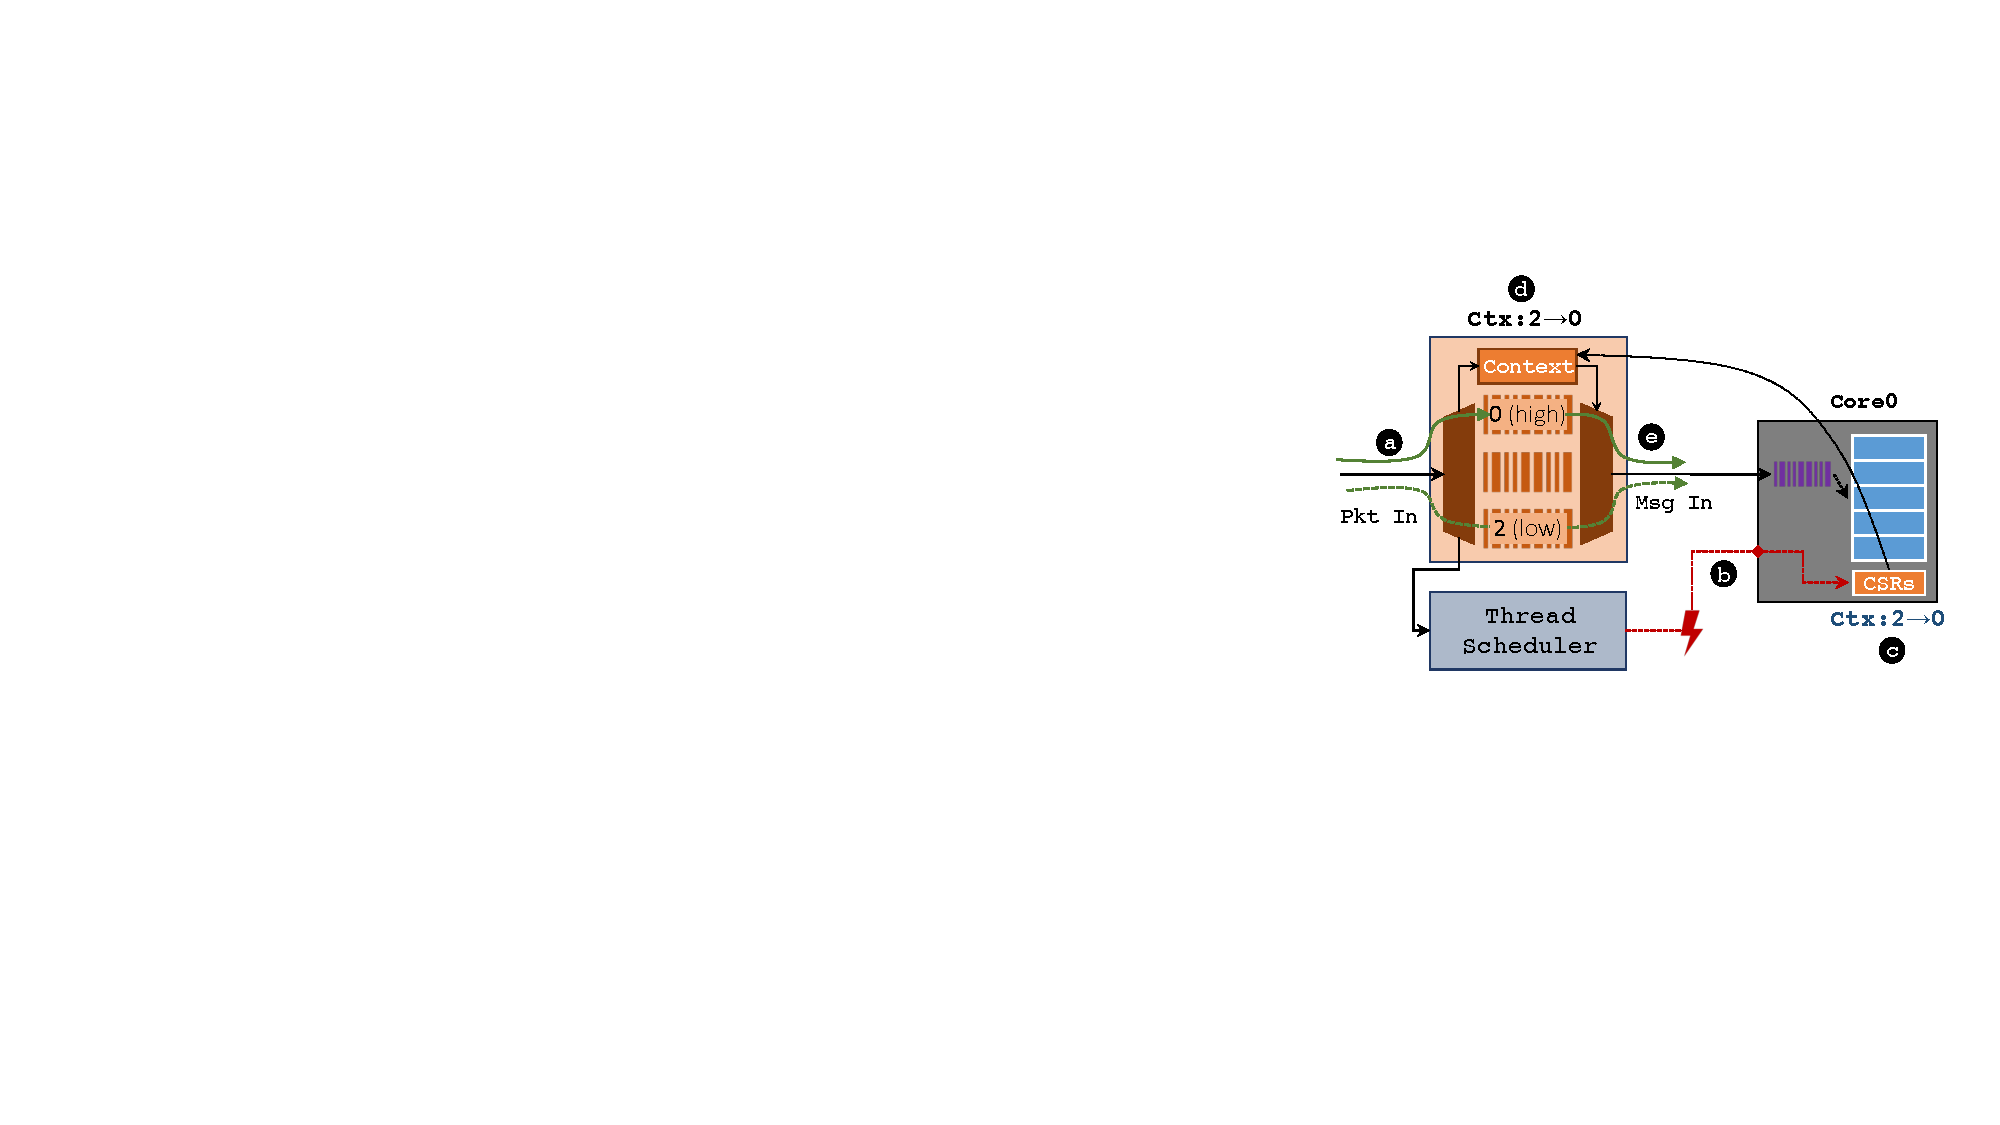
\includegraphics[width=0.8\linewidth]{./figures/thread-sched}
  \caption{The steps that occur when a low-priority thread running on a core is preempted by a higher-priority context.}
  \label{fig:nic-scheduler}
\end{figure}